% ----------------------------  START --------------------------- 
\documentclass[../main]{subfiles} % main refers to main.tex
\graphicspath{{\subfix{../Illustrations}}}
\begin{document}
\addto\extrasfrench{\protected\edef:{\unexpanded\expandafter{:}}}
\selectlanguage{french}
% --------------------------------------------------------------- 

\begin{figure}[ht]
    \centering
    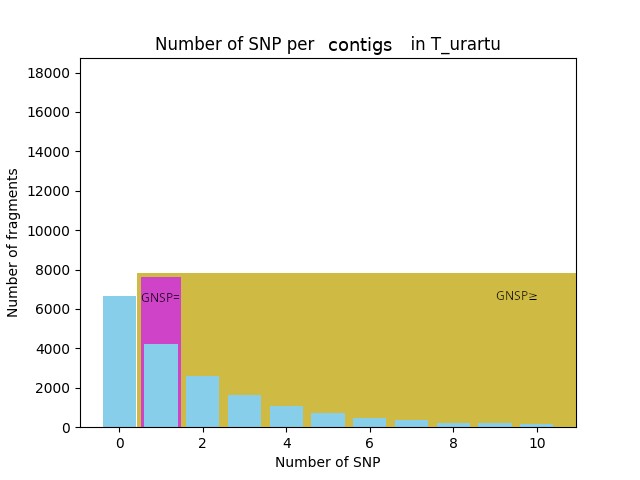
\includegraphics[width=0.9\textwidth]{../Illustrations/ExempleTriticum.png}
    \caption{Exemple de sortie de \cref{sec:SnpHeatmap}. La zone violette représente la partie prise en compte par \GNSPeq tandis que la zone jaune représente le \GNSPge. Cette zone s'étend aussi en dehors des limites du graphique. L'abscisse représente le \NbSNP et l'ordonnée représente le nombre de \contigs présentant ce \NbSNP. Cette image a été générée en même temps que la \cref{fig:SNPHeatmap} et correspond au graphique quantitatif de \textit{Triticum urartu}. La figure a été modifiée en utilisant \gimp.}
    \label{fig:ExempleTriticum}
\end{figure}


% --------------------------------------------------------------- 
\end{document}
% ----------------------------  END --------------------------- 
